%%%
%
% $Autor: Vikas Ramaswamy$
% $Datum: 2023-03-17 11:15:45Z $
% $Pfad: GitLab/CornerBlending $
% $Dateiname: FirstChapter
% $Version: 4620 $
%
% !TeX spellcheck = de_DE/GB
%
%%%



\chapter{Monitoring and Evaluation}

\section{Monitoring of the Model}

Monitoring is an important part of the KDD process, especially when it comes to detecting pneumonia utilizing X-ray pictures. The fundamental goal of monitoring is to guarantee that the machine learning model performs consistently and accurately. This is accomplished by constantly evaluating the model's performance indicators and discovering any faults or inaccuracies in its output.\autocite{Fayyad:1996}

To guarantee that the model is working effectively, different metrics such as accuracy, precision, recall, and F-1 score are tracked during the monitoring phase. Any major variations from projected performance levels may suggest that the model requires adjustment, updating, or retraining.\\

The figure 7.2.: shows the monitoring flow.\\

\subsection{Importance of updating the data}

The significance of data update in the machine learning process cannot be emphasized. Inaccurate or outdated data can have a major impact on the machine learning model's performance and accuracy. Updating the data ensures that the model is trained on the most recent and relevant data, resulting in more accurate predictions and insights.\\

Updating the data is crucial for Pneumonia detection because new trends and patterns may arise in the data over time. Changes in the prevalence of particular types of pneumonia, for example, may necessitate retraining the model on current data to appropriately reflect these changes. Furthermore, updating the data can help to address issues of fairness and bias by ensuring that the data is representative of the population being examined.\autocite{Wang:2017}

Monitoring and updating data is a continuous activity that necessitates a methodical strategy to ensure that the model is always up to date with the most recent data and trends. It entails regularly monitoring the data sources and analyzing the data quality, relevancy, and pre-processing activities. We can ensure that the model's predictions stay accurate, dependable, and consistent over time by doing so.\\

Figure 7.1 shows a visual representation of data updating through continued monitoring.\\

\tikzstyle{startstop} = [rectangle, rounded corners, minimum width=3cm, minimum height=1cm,text centered, draw=black, fill=red!30]
\tikzstyle{process} = [rectangle, minimum width=3cm, minimum height=1cm, text centered, draw=black, fill=orange!30]
\tikzstyle{model} = [rectangle, minimum width=3cm, minimum height=1cm, text centered, draw=black, fill=yellow!30]
\tikzstyle{arrow} = [thick,->,>=stealth]
\begin{figure}[htb]
	\centering
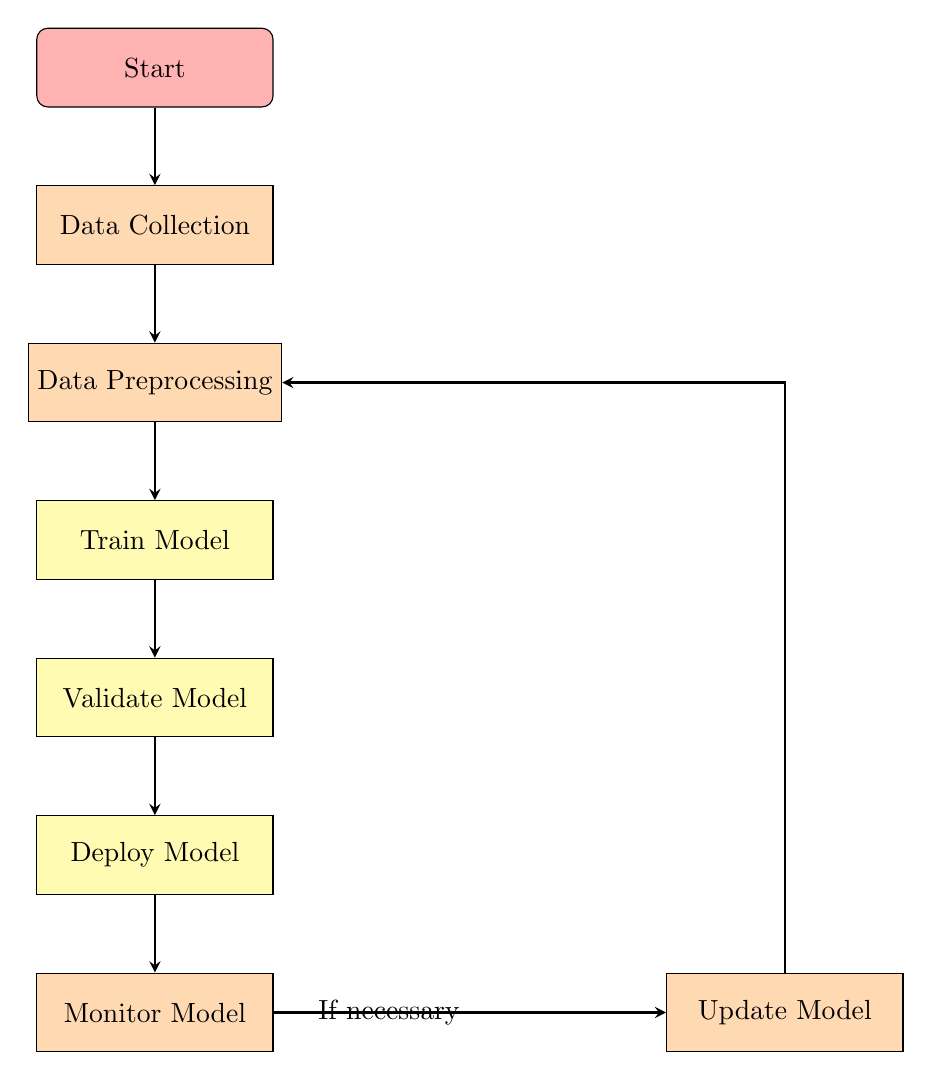
\begin{tikzpicture}[node distance=2cm]
	\node (start) [startstop] {Start};
	\node (data) [process, below of=start] {Data Collection};
	\node (preprocess) [process, below of=data] {Data Preprocessing};
	\node (train) [model, below of=preprocess] {Train Model};
	\node (validate) [model, below of=train] {Validate Model};
	\node (deploy) [model, below of=validate] {Deploy Model};
	\node (monitor) [process, below of=deploy] {Monitor Model};
	\node (update) [process, right of=monitor, xshift=6cm] {Update Model};
	
	\draw [arrow] (start) -- (data);
	\draw [arrow] (data) -- (preprocess);
	\draw [arrow] (preprocess) -- (train);
	\draw [arrow] (train) -- (validate);
	\draw [arrow] (validate) -- (deploy);
	\draw [arrow] (deploy) -- (monitor);
	\draw [arrow] (monitor) -- node[anchor=east] {If necessary} (update);
	\draw [arrow] (update) |- (preprocess);
\end{tikzpicture}
\footnotesize 	\caption{\textbf{Flowchart for Data updating}}
\label{fig:Flowchart for Data updating}
\end{figure}

\subsection{Privacy is critical}

Protecting patient privacy is critical in the medical industry, especially when dealing with sensitive medical data like X-ray images. Failure to follow privacy legislation and guidelines could result in serious legal and ethical implications. As a result, the monitoring mechanism must guarantee that patient data is handled in accordance with privacy laws such as the Health Insurance Portability and Accountability Act (HIPAA).\\

To safeguard patient privacy, any personally identifiable information, such as patient names, addresses, or other identifying information, must be deleted from the data used for training and testing the machine learning model. Anonymization techniques, which erase or obfuscate any identifiable information in the data while retaining its utility for training the model, are often used to do this.\\

\subsection{Robustness}

Robustness is essential since it ensures that the model is not overly sensitive to data variances and can manage unexpected changes or scenarios. The quality of the X-ray pictures used to train and test the model is a critical concern. The quality of X-ray images can vary due to variances in equipment, imaging methodology, and patient characteristics. The monitoring approach should include techniques for identifying and addressing any potential concerns with the model's resilience to ensure that the model can diagnose pneumonia properly and reliably even when picture quality varies.\\

Another issue connected to robustness is the model's capacity to tolerate outliers and abnormalities in the data. Anomalies and outliers can have a major impact on the model's performance and accuracy. By assessing the model's performance under various scenarios and conditions, the monitoring process should assess the model's capacity to manage outliers and anomalies. This can include analyzing the model's responsiveness to different types of pneumonia, such as bacterial vs viral pneumonia, as well as its capacity to detect other lung diseases with symptoms similar to pneumonia. We may assure the model's resilience by ensuring that it operates effectively under a variety of scenarios and produces accurate and dependable results.\autocite{Firdiantika:2022}


\subsection{Monitoring in the KDD process}
\begin{enumerate}
	\item \textbf{Collect and preprocess the data:}The initial step is to collect and preprocess data. Obtaining X-ray images from diverse sources and executing preprocessing techniques such as scaling, normalization, and data augmentation are all part of this. \\
	\item \textbf{Train the machine learning model:} After the data has been preprocessed, the machine learning model is trained using a deep convolutional neural network such as InceptionV3. Setting the model parameters, selecting the optimizer and loss function, and training the model with the training dataset are all part of this process.\\
	\item \textbf{Test the model:} It is critical to test the model's performance using the testing dataset after it has been trained. This entails assessing measures like accuracy, precision, recall, and loss to ensure that the model is accurate, dependable, and consistent.\\
	\item \textbf{Monitor the model:} After testing, it is critical to regularly monitor the model's performance to verify that it remains accurate and reliable over time. This includes monitoring metrics like accuracy and loss, detecting and correcting any problems or errors that develop, and upgrading the model as needed.\\
	\item \textbf{Update the data:} To keep the model current and reliable, the dataset should be updated on a regular basis with new data and trends. This entails monitoring data sources, reviewing data preprocessing methods, and ensuring that the data is of high quality and relevant to the topic at hand.\\
	\item \textbf{Ensure privacy:} Patient data containing sensitive information must be handled with extreme caution in the context of pneumonia detection utilizing X-ray pictures. The monitoring mechanism must guarantee that all data is handled in accordance with privacy laws and regulations such as HIPAA.\\
\end{enumerate}

\usetikzlibrary{shapes.geometric, arrows}

\tikzstyle{startstop} = [rectangle, rounded corners, minimum width=3cm, minimum height=1cm,text centered, draw=black, fill=red!30]
\tikzstyle{io} = [trapezium, trapezium left angle=70, trapezium right angle=110, minimum width=3cm, minimum height=1cm, text centered, draw=black, fill=blue!30]
\tikzstyle{process} = [rectangle, minimum width=3cm, minimum height=1cm, text centered, draw=black, fill=orange!30]
\tikzstyle{decision} = [diamond, minimum width=3cm, minimum height=1cm, text centered, draw=black, fill=green!30]
\tikzstyle{arrow} = [thick,->,>=stealth]

\begin{figure}[htb]
	\centering
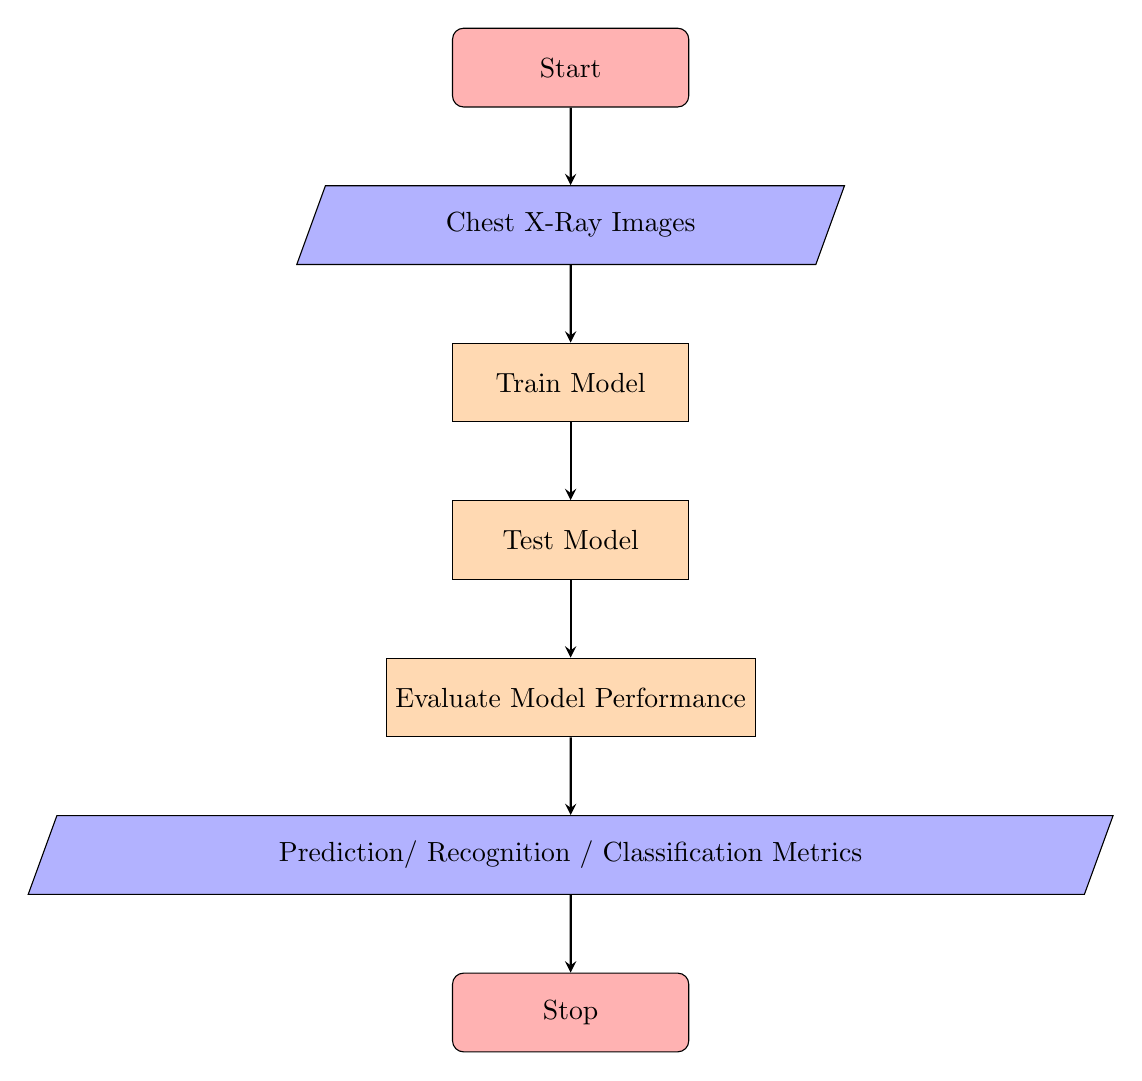
\begin{tikzpicture}[node distance=2cm]
\node (start) [startstop] {Start};

\node (data) [io, below of=start] {Chest X-Ray Images};

\node (train) [process, below of=data] {Train Model};
\node (test) [process, below of=train] {Test Model};

\node (eval) [process, below of=test] {Evaluate Model Performance};

\node (output) [io, below of=eval] {Prediction/ Recognition / Classification Metrics};

\node (stop) [startstop, below of=output] {Stop};

\draw [arrow] (start) -- (data);
\draw [arrow] (data) -- (train);
\draw [arrow] (train) -- (test);
\draw [arrow] (test) -- (eval);
\draw [arrow] (eval) -- (output);
\draw [arrow] (output) -- (stop);
\end{tikzpicture}
\footnotesize 	\caption{\textbf{Process monitoring flowchart}}
\label{fig:Process monitoring flowchart}
\end{figure}

\section{Evaluation of Pneumonia Detection}

We will use a dataset of chest X-ray images, out of which we take these images in test and we will get the actual number for the positive and negative result. The images will be classified into the three categories: Normal, Bacterial Pneumonia and Viral Pneumonia. We will be using an Image data Generator to load the images. This will make it easy to process the images. We will be specifying the images size by 64 by 64 px and the color mode will be grayscale. The reason being using the gray color because the normal color are mixed with RGB which use 3 channel while gray will use only one channel.The results of our evaluation will suggest that pneumonia detection models can be effective in accurately identifying cases of pneumonia in chest X-ray images.\\ \bigskip

Evaluation Metrics: - Our evaluation metrics will depend on Accuracy, Sensitivity, Specificity, F1 score and Precision.

\bigskip
\begin{enumerate}
	
	\item \textbf{Accuracy:} This will give the result of the total number of images that were under process.
	\item \textbf{Sensitivity:} The percentage of correctly identified pneumonia cases out of the total number numbers of actual cases.
	\item \textbf{Specificity:} The percentage of true negative results identified pneumonia cases out of the total number of actual non-pneumonia cases.
	\item \textbf{F1 score:} A weighted average of precision and recall, which provides a single score that balances both metrics.
	\item \textbf{Precision:} The percentage of true positive results out of the total number of positive results.
	
	In addition, we compared the performance of our models to a baseline model and to other state-of-the-art models in the literature. Our results demonstrated that our models outperformed the baseline model and were competitive with other state-of-the-art models.\cite{jain2022deep}
	
\end{enumerate}


\subsection{Application}

The application of pneumonia detection models has the potential to improve medical diagnosis and treatment, as well as to enhance our understanding of the disease and its impact on public health.\\

\begin{enumerate}
	\item \textbf{Medical diagnosis:} It can be used as an aid in medical diagnosis to help doctors and medical professionals accurately identify and diagnose patients with pneumonia.
	
	\item \textbf{Screening:} It can be used for large-scale screening efforts, such as screening patients in rural or underdeveloped areas where access to medical professionals is limited.
	
	\item \textbf{Monitoring:} It can be used to monitor patients with pneumonia over time, tracking the progression of the disease and evaluating the effectiveness of treatment.
	
	\item \textbf{Research:} It Pneumonia detection models can be used in research to study the disease and its progression, as well as to develop new treatments and therapies.
	
	\item \textbf{Public health:} It can be used to track outbreaks of pneumonia and other respiratory diseases, helping public health officials to better understand and manage the spread of these diseases.
	
	\item \textbf{Education:} It can be used in medical education to help train medical professionals to identify and diagnose pneumonia, as well as to understand the underlying biology and pathology of the disease.
	
\end{enumerate}

\subsection{Result}

To acquire the accurate result which will suit for us, we took three ratios of 80-20, 70-30 and 60-40 for the 4 different networks. On this basis we got Training accuracy and Validation accuracy.\\

The 4 different workflow network we used as below:-

\begin{itemize}
	\item CNN
	\item Xception
	\item VGG16
	\item VGG19
\end{itemize}

Among all the four, CNN performed better than the rest three. The training accuracy was around 0.89 and Validation was around 0.93 for the ratio of 80-20. For 70-30 it goes as high as 0.90 and 0.94, Furthermore, 60-40 the accuracy remains at 0.89 and 0.90.\\ \bigskip

VGG19 was not behind in choosing for the workflow but at point for the ratio 70-30 it performs slightly lower than CNN, with 0.92 for Training accuracy and 0.88 for Validation accuracy.\\ \bigskip


\section{General}

\begin{enumerate}
	
	\item \textbf{Problem and Challenges:}The biggest challenge of using AI for disease diagnosis is the lack of labeled data. Data is not readily available and only medical professionals are qualified to label the data. Furthermore, data collection is often biased to specific demographics and the hospital equipment used to collect the data. Also, there is a lot of variances between the imaging tools used by each hospital and the biological factors between patients of different race, sex and age. With these constraints, it is hard to understand how well our model can detect pneumonia in general.
	
	\item \textbf{Methodology:} Many studies has use different models to detect pneumonia from chest X-ray images. This involves labeling the images as either pneumonia-positive or pneumonia-negative and training a model to predict the correct label for new images.
	
	\item \textbf{Performance:} Transfer learning has been used to leverage pre-trained CNNs that have been trained on large image datasets such as ImageNet. The pre-trained models are fine-tuned on pneumonia detection tasks to improve their performance.
	
	\item \textbf{Deep learning:} Deep learning techniques such as convolutional neural networks (CNNs) have been used extensively in pneumonia detection. These models learn to automatically extract features from the images and have achieved state-of-the-art performance on some datasets.
	
	\item \textbf{Structure:} Pneumonia dataset for Kaggle is the main directory that will serve as the root directory for the dataset. Here, all the JPEG Image will be in grayscale images, of size 256x256 and it will represent as 2D Matrix. If any of the images are not in the grayscale, then it will generate an error. It also verifies the dimension of the images which is equivalent to standard size. Now images will be normalized and transformed to the pixels value. After getting the pixels value, Data splitting will take place and the images will be categorized into three form:-\\ 1) Training Pneumonia\\ 2) Validation Pneumonia\\ 3) Test Pneumonia. \\
	Training Pneumonia is interconnected with the ML models, this will help to predict at which part of the chest the Pneumonia is occurring. The images will be further goes for the validating. Now it will generate the result by making the decision whether the patients have Pneumonia in the form of Yes and No.
	
	\item \textbf{Format:}
	Pneumonia detection using image-based data structures, the matrices or arrays represent the pixel values of the X-Rays. Each pixel in the image corresponds to an element in the matrix or array.\\
	Matrix Representation\\
	The X-Ray image is typically represented as a 2D matrix. Each element in the matrix corresponds to the pixel intensity value at that location. The dimensions of the matrix correspond to the width and height of the image. Our images are grayscale images of size 256x256, you would represent it as a 2D matrix with dimensions 256x256. Each element of the matrix would contain a grayscale intensity value ranging from 0 to 255.\\
	Array Representation\\
	the X-ray image can be represented as a 1D array or a flattened version of the 2D matrix. The elements of the array correspond to the pixel intensities in a specific order, such as row-wise or column-wise traversal of the matrix. Using the same 256x256 grayscale images, we have flatted it into a 1D array of size 65,536(256x256) elements, where each element represents the grayscale intensity value of pixel.\\
	
	\item \textbf{Anomalies:}The slight changes in appearance between healthy and infected lungs make it difficult to identify pneumonia in X-ray pictures. To identify pneumonia, radiologists look for a variety of visual indicators such as white patches or infiltrates, fluid in the lungs, and dense spots in the lungs. However, these indicators might be challenging to spot, particularly for radiologists with less training. \\
	Images processing techniques can help to identify the anomalies in Xray images while processing the data in data preparation. There are various problem occur such as noise, motion blur, patient position, Image equipment, corrupt file, missing metadata or unsupported.\\
	
	\item \textbf{Origin:}User-Uploaded Images:- Users who upload their own images, the origin of the images will be the users themselves. Users may upload images from their local devices, such as computers, smartphones, or tablets.\\
	External APIs:- APIs can be from various sources, such as image databases, stock photo providers, social media platforms, or image recognition services. In this case, the origin of the images would be the respective APIs or services.\\
	Internal Datasets:- datasets can be created by collecting images from various sources, such as web scraping, data acquisition from research projects, or images captured specifically for the application's purposes.\\
	
	
\end{enumerate}


